\section*{Цель работы}

\begin{enumerate}
    \item Моделирование и исследование работы JK-, RS- и D-триггеров в LTspice
\end{enumerate}


\section*{Рабочее задание}

В соответствии с вариантом 16 будет реализован асинхронный RS-триггер на ИЛИ-НЕ
логических элементах. Соберем схему RS триггер как на рисунке \ref{fig:rsff_scheme}.
Просимулировав ее можно получить графики сигналов во времени (см. рис. \ref{fig:rsff_signals}).



\begin{figure}[H]
    \centering
    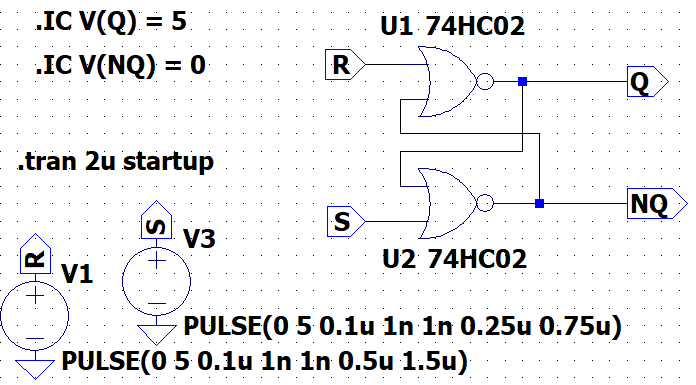
\includegraphics[width=\textwidth]{figs/RSFF_scheme.png}
    \caption{Схема асинхронного RS триггера}
    \label{fig:rsff_scheme}
\end{figure}

\begin{figure}[H]
    \centering
    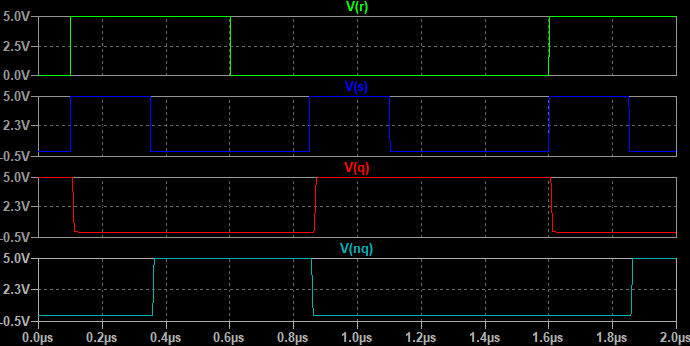
\includegraphics[width=\textwidth]{figs/RSFF_signals.png}
    \caption{Сигналы асинхронного RS триггера}
    \label{fig:rsff_signals}
\end{figure}


По графикам сигналов можно составить таблицу состояний RS триггера (см. таблицу \ref{tab:rsff_table}).
Она полностью совпадает с теоретической.


\begin{table}
    \centering
    \caption{Таблица состояний RS триггера}
    \begin{tabular}{|c|c|c|c|}
        \hline
        $S$&$R$&$Q$&$\overline Q$\\
        \hline
        0&0&$Q_{-1}$&$\overline Q_{-1}$\\
        \hline
        0&1&0&1\\
        \hline
        1&0&1&0\\
        \hline
        1&1&0&0\\
        \hline
    \end{tabular}
    \label{tab:rsff_table}
\end{table}




\section*{Заключение}

В данной лабораторной работе был собран и смоделирован
RS-триггер на микросхемах 74HC02. 
Полученные графики и таблица состояний соответствуют теоретическим.